\documentclass[10pt]{beamer}

\usepackage{multicol}
\usepackage[ngerman]{babel} 
\usepackage{blindtext}
% Zeilenabstände auf 0 setzen
%\usepackage{enumitem}
\usepackage{graphicx}
\usepackage{verbatim}

% Formeln
\usepackage{amsmath,amssymb,amstext,mathabx}

% Schrift
%\renewcommand*\familydefault{\sfdefault}
%\newcommand{\changefont}[3]{\fontfamily{#1} \fontseries{#2} \fontshape{#3} \selectfont}

% Farben
%\usepackage[usenames,dvipsnames]{xcolor}

\usepackage{parcolumns}
\usepackage{pstricks-add}

%Definiere Farben:
\definecolor{orange}{rgb}{1,0.5,0}
\colorlet{notgreen}{blue!50!yellow}
\usepackage{pdfpages}
\usepackage{diagbox}
\usepackage[utf8]{inputenc}
\usepackage[T1]{fontenc}
\usepackage{textcomp}
\usepackage{float}

\bibliographystyle{unsrt}

\setlength{\parindent}{0pt}%gegen Einrücken nach Bildern
\usepackage{pdfpages}%includepdf 
%Fuer die Quellen wird BibLaTeX genutzt:
\usepackage{lmodern}%bibliography
\restylefloat{table}


% some other useful packages
%\usepackage{url}


%%%%%%%%%%%%%%%%%%%%%%%%%%%%%%%%%%%%%%%%%%%%%%%%%%%%%%%%%%%%%%%%%%%%%
%%% my shortcuts
%%%%%%%%%%%%%%%%%%%%%%%%%%%%%%%%%%%%%%%%%%%%%%%%%%%%%%%%%%%%%%%%%%%%%
\newcommand{\highlight}[1]{{\color{blue}\bf#1}}
\newcommand{\todo}[1]{{\color{blue}\bf TODO: #1}}


%%%%%%%%%%%%%%%%%%%%%%%%%%%%%%%%%%%%%%%%%%%%%%%%%%%%%%%%%%%%%%%%%%%%%
%%% setup beamer presentation theme
%%%%%%%%%%%%%%%%%%%%%%%%%%%%%%%%%%%%%%%%%%%%%%%%%%%%%%%%%%%%%%%%%%%%%

\mode<presentation>
{
  \usetheme{TUDortmund2}
}

% include intermediate TOCs automatically at each \section
\AtBeginSection[]
{
  \begin{frame}[c]
    \frametitle{Content}
    \tableofcontents[currentsection]
  \end{frame}
}

% Suppress navigation symbols
\setbeamertemplate{navigation symbols}{}


%%%%%%%%%%%%%%%%%%%%%%%%%%%%%%%%%%%%%%%%%%%%%%%%%%%%%%%%%%%%%%%%%%%%%
%%% titlepage information
%%%%%%%%%%%%%%%%%%%%%%%%%%%%%%%%%%%%%%%%%%%%%%%%%%%%%%%%%%%%%%%%%%%%%

\title{Mixed Precision}
\author{Christoph Höppke, Daniel Tomaschewski}
\institute[TU Dortmund]{TU Dortmund}
\date{Version:\today}



%%%%%%%%%%%%%%%%%%%%%%%%%%%%%%%%%%%%%%%%%%%%%%%%%%%%%%%%%%%%%%%%%%%%%
%%% titlepage
%%%%%%%%%%%%%%%%%%%%%%%%%%%%%%%%%%%%%%%%%%%%%%%%%%%%%%%%%%%%%%%%%%%%%
\begin{document}
% Use non-transparent version of logo for title page
\logo{\centering%

\includegraphics[height=0.5cm]{figures/logo_TUDortmund}%
\hspace*{1em}%

\includegraphics[height=0.5cm]{figures/logo_fakm}%
\hspace*{15em}}
\begin{frame}[c]
  \titlepage
\end{frame}

% no logo from now on, just eats space
\logo{}

\begin{frame}{Content}
\tableofcontents

\end{frame}
%%%%%%%%%%%%%%%%%%%%%%%%%%%%%%%%%%%%%%%%%%%%%%%%%%%%%%%%%%%%%%%%%%%%%
%%%%%%%%%%%%%%%%%%%%%%%%%%%%%%%%%%%%%%%%%%%%%%%%%%%%%%%%%%%%%%%%%%%%%
\section{Mixedprecision Definition and Goals}
%%%%%%%%%%%%%%%%%%%%%%%%%%%%%%%%%%%%%%%%%%%%%%%%%%%%%%%%%%%%%%%%%%%%%
%%%%%%%%%%%%%%%%%%%%%%%%%%%%%%%%%%%%%%%%%%%%%%%%%%%%%%%%%%%%%%%%%%%%%
\subsection{Definition}
\begin{frame}{Definition}
\onslide<1->
\begin{block}{\textbf{Definition:}}
An Algorithm that 
uses different precisions in its computation
\end{block}

%\textbf{Example:} \\Matrix and RHS assembly in double precision\\
%and Solving in single precision
\onslide<2->
\textbf{Goal: } 
\begin{itemize}
\item[] Obtain the \textbf{same accuracy}~by using 
high precision
\item[] but \textbf{better performance}
by utilizing low precision computations
\end{itemize}
\onslide<3->
\textbf{Performance Gains for bandwidth bound algorithms}~\\
 \begin{itemize}
  \item 64 bit = 1 double = 2 floats = 4 halfs
  \item More variables per \textbf{bandwidth} and variables per \textbf{storage}
  \item Applies to all memory levels: network, disc, main, device, local, register 
 \end{itemize}
\onslide<4->
\textbf{Performance Gains for compuation bound algorithms}~\\
 \begin{itemize}
  \item 1 double addition $\approx$ 2 float additions $\approx$ 4 half additions (linear)
  \item 1 double multip. $\approx$ 4 float multip. $\approx$ 16 half multip. (quadratic)
  \item $\rightarrow$ up to 16 times better computational efficiency
 \end{itemize}

\end{frame}




%\subsection{Performance Gains}
%\begin{frame}{Performance Gains}
%\begin{itemize}
%\item \textbf{Bandwidth bound algorithm}
%	\begin{itemize}
%	\item 64 bit = 1 double = 2 floats = 4 halfs
%	\item More variables per \color{red}{bandwidth}\color{black}
%	\item More variables per \color{red}{storage}\color{black}
%	\item Applies to all memory levels: network, disc, main, device, 
%			local, register
%	\end{itemize}
%\item \textbf{Computation bound algorithm}
%	\begin{itemize}
%	\item 1 double addition $\approx$ 2 float additions $\approx$ 4 half 
%			additions (linear)
%	\item 1 double multip. $\approx$ 4 float multip. $\approx$ 16 
%			half multip. (quadratic)
%	\item $\rightarrow$ up to 16 times better computational efficiency
%	\end{itemize}
%\end{itemize}
%\end{frame}

\subsection{Precision}
\begin{frame}{Roundoff and Cancellation}
\onslide<1->
\begin{block}{Definition Machine Precision}
The smalles positive number $\epsilon$ for wich a floating point 
calculations evaluates the expression $1 + \epsilon > 1$ to be true.
\end{block}
\onslide<2->
\textbf{Examples:}
\begin{itemize}
\item $\epsilon_{double} \approx 2.220446049250313\cdot 10^{-16}$
\item $\epsilon_{float} \approx 1.1920929\cdot 10^{-7}$
\item $\epsilon_{half} \approx 9.765625\cdot 10^{-4}$
\item So \color{red}more precision\color{black}~is usually \color{red}better
\end{itemize}
\onslide<3->
\textbf{Cancellation}
\begin{align*}
&\text{additive roundoff } & a=1+0.00000004 &= 1.00000004 &=_{fl} 1\\
&\text{multiplicative roundoff } & b = 1.0002 \cdot 0.9998 &=0.99999996 &=_{fl} 1\\
&\text{\color{blue}cancellation\color{black}~}  &c\in \lbrace a,b\rbrace 
\hspace{1cm}\pm 4 &= (c-1)\cdot 10^8 &=_{fl} 0 \\
&\text{oder~of~operations}  & 1+0.00000004 -1 &=_{fl} 0\\
& &1-1 + 0.00000004 &=_{fl} 0.0000004
\end{align*}
\end{frame}


\begin{frame}{Computational Precision vs Accuracy of Result}
\onslide<1->
\begin{block}{Instructive Example [S.M. Rump, 1988]}
$f(x,y) = (333.75 - x^2)y^6 + x^2(11x^2y^2 - 121y^4-2) + 5.5y^8 + 0.5x/y$\\
$x_0 = 77617, y_0 = 33096$
\end{block}

\begin{align*}
&\text{float s23e8} \hfill &1.1726\\
&\text{double s52e11} \hfill &1.17260394005318\\
%&\text{quad s63e15} \hfill &1.172603940053178631
%&\text{quad s112e15} \hfill &1.172603940053178631
\end{align*}
\onslide<2->
\textbf{The correct result is:}\\
\begin{center}
\color{red}-0.82739605994682136814116509547981629\color{black}
\end{center}
\end{frame}

\subsection{Data Error and Truncation}
\begin{frame}{DataError and Truncation}
\begin{itemize}
\item Data error occurs when the \color{red} exact value~\color{black} has to be \color{red} truncated \color{black} for storage in the binary format
	\begin{itemize}
		\item $\pi$ , $\sqrt{2}$, $sin(2)$, $e^2$, $1/3$
		\item every rational number with a denominator that has a prime 
		      factor other than $2$
	\end{itemize}
\item How can float be better than double?
\begin{itemize}
	\item There is \color{red} no data error \color{black} in the operands
	\item The errors can \color{red} cancel out \color{black} themselves 
		  favorably
\end{itemize}
\color{black}
\end{itemize}

\end{frame}


\subsection{Floting Point Operations. A deeper analysis}
\begin{frame}{Floating Point Operations. A deeper analysis}
\textbf{Number representation}\textbf{$\rightarrow$ almost all numbers have to be truncated}~\\
\begin{table}[H]
 \centering
      \begin{tabular}{l|l|l|l}
	half s10e5~a&\text{1 bit sign $s_a$~}&\text{10 bit mantissa $m_a$~}&\text{5 bit exp. $e_a$}\\\hline
	float s23e8~b&\text{1 bit sign $s_b$~}&\text{23 bit mantissa $m_b$~}& \text{8 bit exp. $e_b$}\\\hline
	double s52e11~c&\text{1 bit sign $s_c$~}&\text{52 bit mantissa $m_c$~}&\text{11 bit exp. $e_c$} 
      \end{tabular}
      %\label{tab:L2-Fehler bei einfachen Dimension-Splitting}
\end{table}

\begin{table}[H]
 \centering
      \begin{tabular}{l||l|l}
	\textbf{Multiplication} & & \\\hline\hline
	Precision & Exactformat & Mantissa truncation: \\\hline\hline
	half(a) $\cdot$ half(b)& s20e6& from 20 to 10 bit \\\hline
	float(a) $\cdot$ float(b)& s46e9& from 46 to 23 bit \\\hline
	double(a) $\cdot$ double(b)& s104e12& from 104 to 52 bit 
      %\label{tab:L2-Fehler bei einfachen Dimension-Splitting}
      \end{tabular}
    \hfill
  \begin{tabular}{l||l|l}
	\textbf{Addition} & & \\\hline\hline
	Precision & Exactformat & Mantissa truncation: \\\hline\hline
	half(a) $\cdot$ half(b)& s41e5& from 41 to 10 bit \\\hline
	float(a) $\cdot$ float(b)& s278e8&  from 278 to 23 bit \\\hline
	double(a) $\cdot$ double(b)& s2099e11& from 2099 to 52 bit 
      %\label{tab:L2-Fehler bei einfachen Dimension-Splitting}
    \end{tabular}
\end{table}

\end{frame}
%\begin{itemize}
%\item Multiplication $float(a) \cdot float(b)$
%	\begin{itemize}
%	\item Operations: $s_a \cdot s_b$,$m_a \cdot m_b$,$e_a \cdot e_b$
%	\item Excat format: s46e9 = s23e8 $\cdot$s23e8
%	\item Main error: Mantissa truncated from 46 bit to 23 bit
%	\end{itemize}
%\item Addition $float(a) + float(b)$
%	\begin{itemize}
%	\item Operations: $e_{diff} = e_a - e_b$, $m_a + (m_b >> e_{diff})$, 
%			normalize
%	\item Exact format: s278e8 = s23e8+s23e8
%	\item Main error: Maintissa truncated from 278 bit to 23 bit
%	\end{itemize}
%\end{itemize}

%\section{History of Mixed Precision in the context of GPGPU calculations}
%\subsection{History of GPGPU}
%\begin{frame}{History of GPGPU}
%
%	\textbf{1999: NVIDIA GeForce 256}\\
%	\begin{itemize}
%	\item Term GPU was coined during the launch
%	\item GPGPU calculations were only achievable by "Hacking the GPU" 
%			(verry cumbersome and error-prone)
%	\end{itemize}
%~\\~\\
%\textbf{2003-2007 First wave of GPU computing}
%\begin{itemize}
%\item Floating point support
%\item Performance improvements
%\item Geforce 8800GT Release (29.October 2007)\\
%	first CUDA enabled Consumer GPU
%\item Double precision was not available on the GPU
%\item Mixed Precision was the ONLY way to utilize GPU horesepower
%	without precision compromises
%\item Mixed Precision lead to a speedup of factor 3-5 in FEM applications %[http://www.mathematik.tu-dortmund.de/~goeddeke/pubs/pdf/Strzodka_2006_MPM.pdf]
%\end{itemize}
%\end{frame}

\subsection{Why Mixed Precision is difficult}
\begin{frame}{Why Mixed Precision is difficult}
\begin{itemize}
\item Data has to be transferred to the GPU (usually) over the relativly \color{red} slow PCIe \color{black} interface
\item A lot of time is wasted while waiting for data
\end{itemize}
\begin{center}
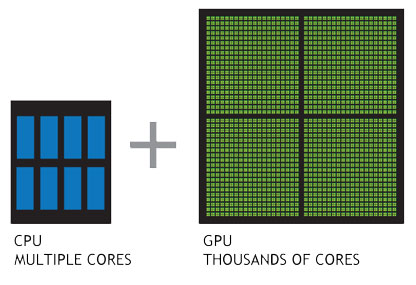
\includegraphics[width=0.5\textwidth]{../SourcesCites/cpu-and-gpu.jpg} 
\end{center}


\end{frame}

\begin{frame}{A brief history overview}
\textbf{Trends:}\\
\begin{itemize}
  \item Memoryclock speeds are increasing\\
  \begin{itemize}
    \item GTX 980 Ti Memoryclock speed: 2x 1753 MHz
    \item GTX 1080 Memoryclock speeds: 4x 2500 MHz (\color{red} +185\%\color{black})
  \end{itemize}
  \item Unconventional computation Hardware\\
  \begin{itemize}
    \item APU's
    \item SOC's such as the NVIDIA Tegra K1
  \end{itemize}
  \item New technologys\\
  \begin{itemize}
   \item Unified memory
   \item NVIDIA pushing the use of half precision by implementing support for half and half2 in CUDA Toolkit version 7.5 
  \end{itemize}
\end{itemize}
\textbf{$\rightarrow$ Sharing memory between CPU and GPU is becoming easyer and more effective}
\end{frame}

\begin{frame}{A brief history overview}
 \textbf{Past achievements:}~\\
\begin{center}
  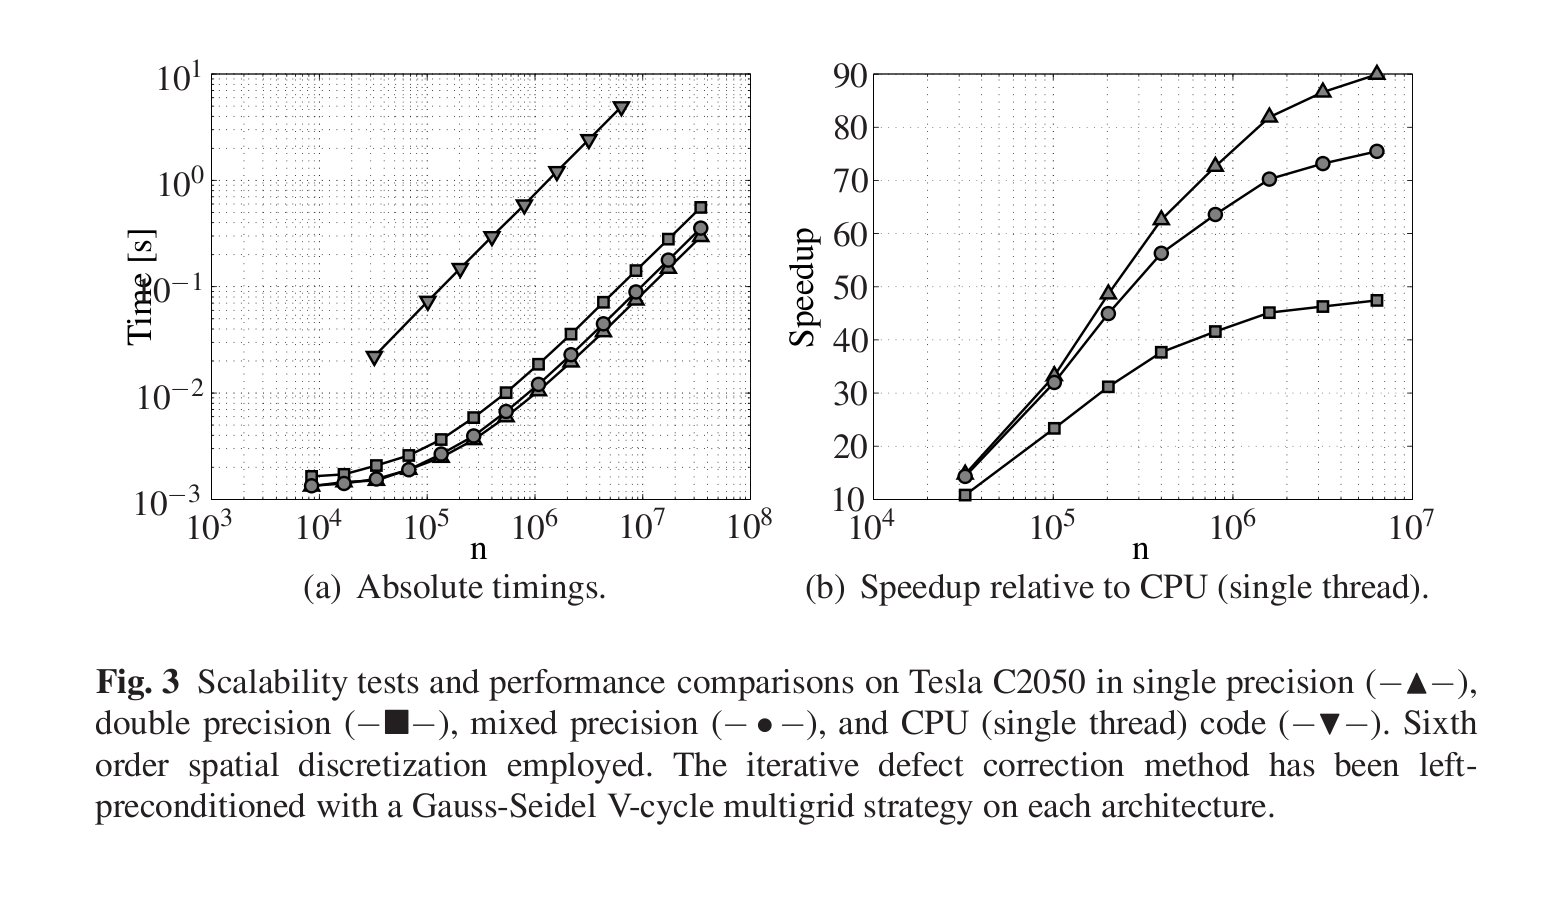
\includegraphics[width=0.9\textwidth]{../SourcesCites/past.jpg}
  \cite{WaterWaveComp}
\end{center}
\textbf{$\rightarrow$ about 35\% performance increase by using mixedprecision}
\end{frame}

%\subsection{Unconventional computation Hardware}
%\begin{frame}{Unconventional compuation Hardware}
%\textbf{NVIDIA Jetson TK1 Bord}
%\begin{itemize}
%\item CPU and GPU share the same memory and use the same memory interface
%\item Copying data from CPU to GPU and vice versa is much faster
%\end{itemize}
%\end{frame}

\section{Example Calculation}
\begin{frame}{Example Calculation}
\begin{block}{Problem}
Solve the Poission problem $- \Delta u = 1,~x\in\Omega$ with dirichlet boundry conditions $u \equiv 0,~x\in \partial \Omega$ using conforming quadrilateral 
elements for the finite-element discretization of the unit square $\Omega = (-1,1)^2$
\end{block}

\begin{itemize}
\item Method 1: Using double precision
\item Method 2 : Using iterative refinement
\end{itemize}
\end{frame}



\subsection{Testresults}
\begin{frame}{Testresults pending}
\begin{center}
\color{red} Imagine a nice Plot\color{black}
\end{center}
\end{frame}
\begin{frame}{Bibliography}
  \bibliography{literaturscout24.bib} 
\end{frame}


\end{document}